\chapter{Conceptual Outline of Our Emulator Code and Pipeline}
\label{chap: cassL}

Now that we have a solution which allows integration of massive neutrinos
into the evolution mapping framework, we are ready to plan and build the
machinery which leads to an emulator. CL represents a full emulation pipeline from the generation of training and 
testing data to the plotting of error statistics associated with
the emulation. This chapter will concentrate on an accessible 
description of the pipeline, motivations behind several key components, as
well as a more detailed and technical breakdown of the implementation of
the steps.

We will name functions with which the
reader will need to be familiar in order to train an accurate emulator with
CL, as well as their limitations and the assumptions they make about their
inputs. Therefore, this chapter contains information necessary even if the
reader is interested only in using and not in modifying CL.

CL may be installed in the fashion typical of Python packages: after cloning
the repository\footnote{https://github.com/3276908917/Master}
or downloading and unzipping it, the command

\verb|pip install -e .|

should be run in the top-level directory (``Master'') and in the
appropriate environment (when using a package manager such as Anaconda).
The reader should keep in mind that we refer to the package as CL in this
thesis to clearly distinguish it from the Boltzmann solver CLASS, but its
true name (for example, for use in \texttt{import} statements) is
\texttt{cassL}.

\section{Pipeline}
\label{sec: flow_chart}

% Disgusting hack to get verbatim functionality in tabel

In this section we outline the general procedure for building and testing an
emulator. For an explanation of the abbreviations used here, see table~\ref{tab: script_summary}. 

\textcolor{red}{The following two paragraphs are not very easy to read, but 
I'm not sure how to better structure them.}

First, the user needs to decide on the desired properties and domain of the
emulator. Most of these properties are currently set within a ``scenario
file.'' Over what range in each parameter should the emulator be trained?
The user should specify these with a priors file (see section~\ref{sec: 
lhc_outline}) and reference it in the scenario file. At how many points in
$k$ should CL predict the power spectrum? By default, we pick $N_k = 300$. 
Where are the training and testing $\matr{X}$ stored?
Does this scenario share an
already-computed test set with a different emulator? For example, one could
re-use a test set built from an 3000 training samples to test an emulator 
built from 7000 training training samples.

When using \texttt{lhc} to generate the training and testing
$\matr{X}$, remaining questions are answered: how evenly does the parameter
space need to be sampled? This involves setting a threshold value for $s^*$,
the minimum separation between any $\bm{x}_1, \bm{x}_2 \in \matr{X}$.
How many samples should each data set have? By default, we pick $N_s = 5000$.

\texttt{ui} processes the scenario file and loads the
$\matr{X}_\text{train}$, $\matr{X}_\text{test}$
and priors into
memory, packaging them into a data dictionary. Before submitting this
dictionary to \texttt{te}, \texttt{ui} requests the power spectra from
\texttt{ged}, which constitute our $\matr{Y}_\text{train}$ and
$\matr{Y}_\text{test}$.\footnote{\texttt{ged} also 
produces the rescale parameters files which are not
necessary for building the emulator but which contain useful diagnostic
information when verifying the correctness of the code. To learn about rescale
parameters, refer to section~\ref{sec: generate_emu_data}}. \texttt{ged}
applies the technique of evolution mapping in interacting with \texttt{ci}.
Finally, \texttt{ged} slightly modifies the $\matr{X}$ to minimize
computational expense (see again section~\ref{sec: generate_emu_data}). 

At this point, we have $\matr{X}_\text{train}$, $\matr{X}_\text{test}$, 
$\matr{Y}_\text{train}$, and $\matr{Y}_\text{test}$. These elements are
organized into a data dictionary and passed to \texttt{te}, which instantiates
a new emulator trainer object. This trainer in turn instantiates an emulator 
object and trains the Gaussian process it contains. Finally, the trainer 
calculates some simple error metrics according to the provided test set.

As a digestible visualization of the procedure as described here, we
include figure~\ref{fig: flow_chart}.

\textcolor{orange}{The emulator should also compute training errors!! This
would be a really easy way to expand the code in a meaningful way.}

\section{Latin Hypercube Sampling}
\label{sec: lhc}

We use Latin hypercube sampling to sample 
the space of cosmological configurations.
A unit Latin hypercube sample (LHS) is primarily characterized by its 
dimension $d$ and number of samples $N_s$. A number $d$ of separate intervals, 
all running from zero to unity, are
each split into $N_s$ subintervals. Then, each subinterval is sampled
exactly once. By contrast, simple random sampling (SRS) may sample any 
particular subinterval any number of times, including not at all. SRS
can require vast numbers of samples before all regions of the space are
represented. For a pictorial representation of SRS versus Latin hypercube
sampling, see figure~\ref{fig: sample_comparison}.

% The following plots were generated with h_units_bad.ipynb
\begin{figure}[ht!]
    \begin{subfigure}{0.32 \textwidth}
    \centering
 		\includesvg[width=\textwidth]{lhs/random}
 		\caption{}
 		\label{fig: random_sample}
    \end{subfigure}
    \begin{subfigure}{0.32 \textwidth}
    \centering
 		\includesvg[width=\textwidth]{lhs/bad_LHS}
 		\caption{}
 		\label{fig: poor_lhs}
    \end{subfigure}
    \begin{subfigure}{0.32 \textwidth}
    \centering
 		\includesvg[width=\textwidth]{lhs/better_LHS}
 		\caption{}
 		\label{fig: better_lhs}
    \end{subfigure}
    \centering
    \caption[Comparison of SRS and Latin hypercube sampling.]{Comparison of an 
    example
    	random sample with two examples of LHSs.
    	\ref{fig: random_sample} a random sample.
    	Some subintervals are sampled repeatedly.
	\ref{fig: poor_lhs} An LHS with a low $s^*$.    	
    	\ref{fig: better_lhs} A different LHS with a higher $s^*$.
    	Unlike random sampling,
    	Latin hypercube sampling guarantees that every subinterval will be 
    	sampled. However, if
    	the minimum separation is low enough, there will still be large
    	undersampled regions.}
    \label{fig: sample_comparison}
\end{figure}

Latin hypercube sampling does not always improve significantly over SRS. It is 
convenient to
assess the quality of an LHS according to the minimum separation $s^*$ 
between any two sample points in the LHS. A high $s^*$ indicates that 
the sample space is evenly covered. To visually appreciate the difference 
between LHSs of different $s^*$ values, see again
figure~\ref{fig: sample_comparison}.

For each value of $d$ and $N_s$, there is a theoretical maximum value of
$s^*$:

\begin{equation}
\label{eq: best_lhs_sep}
s^*_\text{best} = \left( \frac{1}{N_s} \right)^{1 / d}
\end{equation}

For example, for a six-parameter emulator trained over 5000 samples, the best
possible LHS sample would have $s^* \approx 0.2418$.
\textcolor{orange}{Talk about how you got this equation?}

The LHSs give the values of the cosmological parameters and therefore
the give the inputs over which we train the emulator.
Therefore, we referred to the LHSs as the
$\matr{X}$ data sets in the previous section. Each
row $\bm{x}$ in $\matr{X}$ will describe a different cosmology, and each
row $\bm{y}$ in $\matr{Y}$ will be the power spectrum for that cosmology.

Once we generate a unit LHS, we can rescale each coordinate according to a 
different parameter's prior to map the LHS into our parameter space.
These unit LHSs are saved as
\texttt{npy} files and later rescaled according to priors in order to
specify the training
domain in each parameter. This two-step process, first of generating a unit
LHC and then rescaling it, allows us to build many different emulators from a 
single LHS file. That is, rescaling the same LHS in different ways allows us
to cut down on the number of LHSs that we need to generate.

% Intro sentence?

% One reason this goes here: priors show up in almost every script,
% so there isn't a great cass-L section in which to put this.

CL accomplishes this rescaling through the use of priors files.
CL is packaged with two pairs of priors files (the pairing will be explained
in section~\ref{sec: 2emu_intro}). The parameter domains for each pair are
described in tables~\ref{tab: CLASSIC_priors} and~\ref{tab: COMET_priors}. The two pairs of files share the same priors in
$\omega_\nu$, [0, 0.01], and $\tilde{\sigma}_{12}$, [0.2, 1], and so these are
omitted.

\begin{comment}
\begin{table}[ht!]
\centering
\begin{tabular}{l|l|l}
\hline
Parameter & Minimum Value & Maximum Value \\ \hline
$\omega_b$ & 0.005 & 0.28 \\
$\omega_c$ & 0.001 & 0.99 \\
$n_s$ & 0.7 & 1.3 \\
$A_s$\footnotemark & $5.003 \cdot 10^{-10}$ & $1.484 \cdot 10^{-8}$  \\
\end{tabular}
 \cprotect\caption[``MEGA'' priors]{``MEGA'' priors. The range of allowed
 	values is significantly larger than the modern $3\sigma$ intervals
 	for these parameters. It was created from the most extreme values used
 	in table 1 of \citet{Mancini} and table 1 of \citet{Arico}, even including
 	CMB emulators. 
 	\textcolor{red}{Maybe since we didn't end up using this prior file, I
 	should scrap it from the discussion?}}
 \label{tab: MEGA_priors}
\end{table}
\end{comment}

\begin{table}[ht!]
\centering
\begin{tabular}{l|l|l}
\hline
Parameter & Minimum Value & Maximum Value \\ \hline
$\omega_b$ & 0.01875 & 0.02625 \\
$\omega_c$ & 0.05 & 0.255 \\
$n_s$ & 0.84 & 1.1 \\
$A_s$\footnotemark & $1.049 \cdot 10^{-9}$ & $4.990 \cdot 10^{-9}$  \\
\end{tabular}
	\cprotect\caption[``CLASSIC'' priors]{``CLASSIC'' priors. Despite
 	significantly smaller ranges than table~\ref{tab: MEGA_priors}, this
 	parameter space is still easily large enough to accommodate modern
 	statistical analyses. \textcolor{green}{citation.}}
 \label{tab: CLASSIC_priors}
\end{table}

\begin{table}[ht!]
\centering
\begin{tabular}{l|l|l}
\hline
Parameter & Minimum Value & Maximum Value \\ \hline
$\omega_b$ & 0.0205 & 0.02415 \\
$\omega_c$ & 0.085 & 0.155 \\
$n_s$ & 0.92 & 1.01 \\
$A_s$\footnotemark & $1.049 \cdot 10^{-9}$ & $4.990 \cdot 10^{-9}$  \\
\end{tabular}
	\cprotect\caption[``COMET'' priors]{``COMET'' priors.
	These values are significantly more restrictive than in
	tables~\ref{tab: MEGA_priors} and~\ref{tab: CLASSIC_priors},
	but the parameter space should still be large enough to accommodate
	most modern statistical analyses. \textcolor{green}{citation.}
	These priors were taken from table 2 of \citet{Eggemeier}.}
 \label{tab: COMET_priors}
\end{table}

\textcolor{orange}{Talk a little more about the prior ranges, what are their
values in words?}

At first, we used the ambitious ``CLASSIC'' set of priors
(table~\ref{tab: MEGA_priors}), whose values we decided based on the recent 
emulator papers from \citet{Mancini} and \citet{Arico}.
However, during the process of generating training data, 
we found that CAMB was occasionally unable to compute the power spectrum for
all the resulting cosmologies (this issue will be explained in
section~\ref{sec: generate_emu_data}). We do not recommend the use of this
file because the priors are not representative of the ranges appearing in the
training set.

By contrast, the ``COMET'' priors (table~\ref{tab: COMET_priors}) are 
entirely solvable. For this reason and for the cheaper (by number of samples) 
accuracy that comes with tighter priors, the COMET priors are the defaults for 
CL.

The user is welcome to write sets of priors suitable to different 
applications.
To do so, one need only create a new prior file. The format is very simple, 
but must be followed carefully for the file to be read correctly. We
recommend copying one of the existing priors files as a template. 

%%% Ran out of time to implement this feature
\begin{comment}
As one final note on the general implementation of LHSs in CL, we note that
all axes of our \textit{unit} LHSs run \textit{uniformly} over the interval
[0, 1]. However, the rescaled 
parameter domains can be more flexible. For example, the fourth axis
of an LHS
describes $\tilde{\sigma}_{12}$ in the default implementation of the code. We can also
interpret the axis as a set of $\tilde{\sigma}_{12}^2$ values instead,
in case we wish to
increase our sampling in larger values of $\tilde{\sigma}_{12}$ over the same
interval. Unfortunately, this non-uniform sampling does not seem to be
correctly implemented
in the current (as of 2 October 2023) version of the code. Nonetheless, as we
will repeat in section~\ref{sec: future_work},
the feature is in principle simple to implement.
\end{comment}
%%%

Each entry $\bm{x}$ in our LHS $\matr{X}$ will be either a four- or
six-dimensional vector, 
depending on the emulator's support for massive neutrinos. When building a
massless-neutrino emulator, each $\bm{x}$ will describe the $\omega_b$,
$\omega_c$, $n_s$, and
$\tilde{\sigma}_{12}$ values for a different cosmology in 
this order. When building a massive-neutrino emulator, each $\bm{x}$ will 
additionally specify the $A_s$ and $\omega_\nu$ values for that cosmology, 
again in this order.

To generate the LHS, we begin by invoking the \texttt{lhs} function of
\texttt{pyDOE2} a number of times. Each time we get a random new unit LHC, 
whose spacing we analyze with the \texttt{cdist} function from
\texttt{scipy.spatial.distance}. Recall that
our samples more evenly cover the sample space if the minimum separation
$s^*$ increases. Therefore, from among the numerous calls of \texttt{lhs} we 
select the LHS with the largest minimum separation.

In order to maximize the number of random hypercubes generated per unit of
wall time, we have written a multithreaded function called
\verb|multithread_unit_LHC_builder|.
Through the function parameter \verb|num_workers| the user is free to assign
any number of CPU threads to the task; in principle, a CPU can be
wholly dedicated to the optimization of the LHS.
This function lacks a return statement but
instead triggers an unending query for LHSs. The user is notified via command
line printout whenever an LHS has been generated whose $s^*$ exceeds
the previous record. Whenever such a superior LHS is
encountered, the function writes the LHS to a file and continues. Therefore,
the user may run this script in the background and terminate whenever. The
function always writes LHSs to the same file, so each new record-setting LHS
overwrites the old one. When the user terminates the function, whatever output
file remains represents the best LHS seen since the function was first called.

%%% It's just too much detail for a master's thesis, no one will care
\begin{comment}
The \verb|cdist| function can be re-used to compare LHSs loaded from 
different
files. However, since there is generally little reason to keep old LHSs
(except, perhaps, to reconstruct specific emulators), it reduces clutter to
simply continue overwriting the same file. Therefore, the function
\verb|multithread_unit_LHC_builder| also includes a parameter
\verb|previous_record|, which is recommended whenever the user would like to
stop the function and then resume it later. In such a case, the parameter
should be set to the \verb|cdist| value of the exis}
\end{comment}
%%%

% I've got a better idea: the function should automatically ask the user if
% he's sure, in the case that we find a file under the name under which we
% intend to write. If the user is sure, we take the cdist of that existing
% file and use it as the previous record!

% we multithreaded the Python script to spawn 12 workers on an 11th gen Intel 
% i7-11700 @ 2.50 GHz. IF YOU ARE USING THE WORK DESKTOP

As of 2 October 2023, CL relies on this brute-force approach to build the
LHSs that are eventually used to train the emulators. To understand the 
computational and wall-time costs associated with this solution, we include 
figures~\ref{fig: wall_time} and ~\ref{fig: function_calls}.

% The following plots were generated with h_units_bad.ipynb
\begin{figure}[ht!]
    \begin{subfigure}{0.45 \textwidth}
    \centering
 		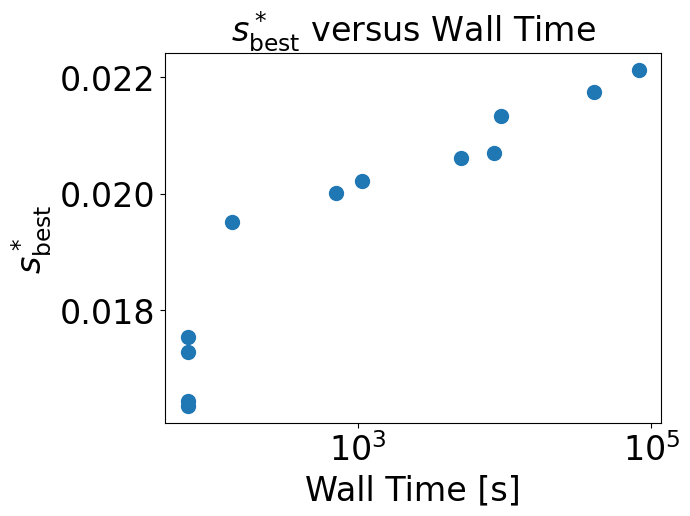
\includegraphics[width=\textwidth]{CL/wall_time}
 		\caption{Using $h$ units.}
 		\label{fig: wall_time}
    \end{subfigure}
    \begin{subfigure}{0.45 \textwidth}
    \centering
 		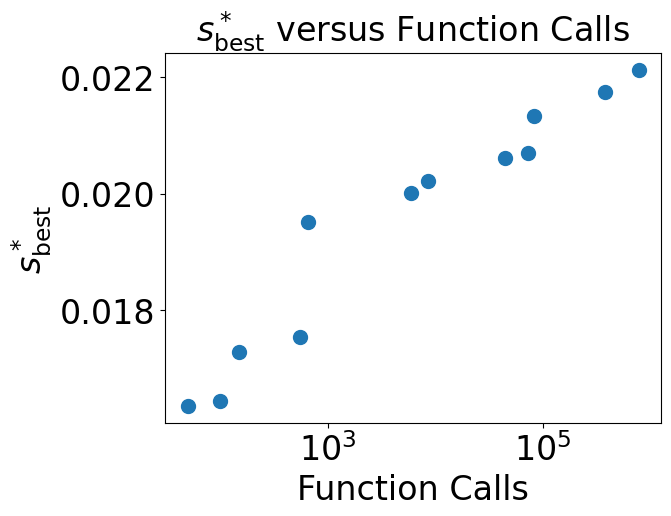
\includegraphics[width=\textwidth]{CL/fn_calls}
 		\caption{Using absolute units.}
 		\label{fig: function_calls}
    \end{subfigure}
        \centering
    \caption[Efficiency of Brute-Force LHS Approach]{We multithreaded our 
    		Python script to spawn 12 workers on an 11th-generation Intel
    		i7-11700 running at 2.50 GHz. After leaving the workers to generate
    		new random LHSs for approximately 50 hours, we measured the progress
    		in two plots. Figure~\ref{fig: wall_time} shows the wall-time cost of
    		reaching a particular $s^*$, while figure~\ref{fig: function_calls}
    		shows this cost through the number of function calls. This second
    		metric will be more useful to users as a system-agnostic example of
    		the cost. However, due to the random nature of LHS generation, these
    		results should be recognized as only an example outcome.}
    \label{fig: random_lhs_performance}
\end{figure}

\begin{comment} % The following paragraph says this stuff better
we left the system to run for two days. In this time, the 
largest minimum separation that we generated was approximately 0.08022.  
Recall from section sec_B1 that the theoretical best possible value for this 
setup is approximately 0.24183. It would have been more meaningful if you had 
counted the total number of function calls, but it isn’t too late to set up 
such a run. So, even after assigning a relatively large amount of compute to 
this brute force solution, we fail to obtain an LHC of even a third of the 
best minimum separation.
\end{comment} 

Recall that equation~\ref{eq: best_lhs_sep}, tells us the best possible $s^*$
given dimension $d$ and total number of samples $N_s$. Let us consider a 
massless-neutrino emulator (a total of four dimensions per cosmology vector)
trained over five-thousand CAMB spectra. If we plug in $d = 4$ and $N=5000$,
we find $s^*_\text{best} \approx 0.1189$. Clearly, the brute force method
achieves only a comparatively low $s^*$, even over the span of multiple days.

Based on figures~\ref{fig: wall_time} and~\ref{fig: function_calls}, we
claim that our approach is inefficient and not well-suited to the task of 
maximizing $s^*$. Since suboptimal $s^*$ values imply unevenness in the
coverage of the space of cosmologies, we expect low $s^*$ values to impact
the emulator by increasing variance in the errors, because the worst errors
will be significantly worse, while the best errors will be slightly better in
oversampled regions. We also expect the average error to increase slightly,
as the oversampled regions should benefit less than the undersampled regions
suffer. We will test these expectations in section~\ref{sec: error_from_lhc} 
by varying the $s^*$ of the LHS with which we train the emulator.

% One could argue that the variance in oversampled regions will decrease to
% compensate, right? I need to clarify that the decrease in variance in the
% oversampled regions would not be able to compensate the increased variance
% in the undersampled regions, because the space of power spectra is
% continuous, so closely spaced points reveal less about the true function
% than well spaced points.

Now that we have a unit LHS $\matr{X}_u$, we need to scale it 
so that each axis, which currently runs from zero to one, runs along a range 
dictated by one of the priors. This scaling is handled by the \texttt{ged}
function \verb|build_cosmology|. It accepts as parameters the values of
$\omega_b$, $\omega_c$, $n_s$, $\sigma_{12}$, $A_s$, $\omega_\nu$, and, 
optionally, a dictionary of priors. If this
dictionary is not provided, the cosmological parameters are assumed to
already have been scaled. When building a massless-neutrino emulator,
the information $\omega_\nu = 0$ and $A_s = A_s(\text{Aletheia model 0})$ is
automatically provided to \verb|build_cosmology| by
\verb|fill_hypercube|. 
% We really should redo build_cosmology so that it assumes indices match to
% the same parameters every time! This is how the rest of the code works,
% after all.

The precise form of the scaling is given by the formula for transforming a
random variable $x \sim \mathcal{U}(0, 1)$ to a random variable
$x' \sim \mathcal{U}(a, b)$:

\begin{equation}
\label{eq: scaling}
x' = x (b - a) + a
\end{equation}

After scaling the parameters, \verb|build_cosmology| finishes bridging the gap
between the LHS and the CAMB \verb|pars| object (as introduced in
chapter~\ref{chap: CAMB_setup}) by using default values to fill in the
remaining values demanded by CAMB. For example, $H_0$, $w_a$ and $w_0$ are
not parameters over which we train the emulator, but CAMB requires that they 
be specified before a power spectrum can be calculated. In all such cases, we 
use Aletheia model 0 as default values. So long as the power spectrum's value 
for $\sigma_{12}$ agrees with the prior-scaled value from the LHS, it should 
not matter that we use the model 0 values, as these are evolution parameters.
\textcolor{orange}{I'm not referring to table 1.2 here
because I would have to expand it with parameters not essential to this work,
so I would have to redo the captions for fig 1.1 and table 1.2...}


\section{Creation of Separate Emulators}
\label{sec: 2emu_intro}

One potential weakness of this emulator outline emerges 
from the prior range for the physical density in neutrinos. The lower bound 
($\omega_\nu = 0$) of this range for the physical density in neutrinos is 
highly firm; any negative value would be unphysical. However, this 
lower bound is also inclusive in the sense that the massless neutrino case is  
of interest to us. GP predictions are, naturally, at their 
strongest for points surrounded with training samples. Since the massless 
neutrino case represents the end of a parameter range, there will by 
definition be no samples in the $\omega_\nu < 0$ direction with which to
interpolate. Indeed, due to the nature of random sampling (including both 
Latin hypercube and simple random sampling), we do not expect \textit{any}
of our
samples to be located exactly at $\omega_\nu = 0$.
Therefore, we expect the massless-neutrino case to be a slight
\textit{extrapolation} from our training data, which is dangerous for 
accuracy.

%%% Footnote just opens you up to even worse questions
\begin{comment}
\footnote{\textcolor{orange}{What should I say to people who complain: 
``why not just manually add massless-neutrino samples to the original training 
set? Why not simply have one emulator trained over a more diverse training 
set?'' I think it would be better if we simply focus on the $\omega_\nu = 0$
case not being adequately captured by interpolation, since we don't have any
samples on the ``left'' side of $\omega_\nu = 0$.}}
\end{comment}
%%%

To address this unique problem among our parameter ranges, we train two
independent CL emulators. The primary 
emulator is trained over the aforementioned prior range,
$\omega_\nu \in [0, 0.01]$, with $A_s$ depending on the priors file used
(see tables~\ref{tab: MEGA_priors},~\ref{tab: CLASSIC_priors},
and~\ref{tab: COMET_priors}). The secondary emulator is specifically trained
to handle the massless neutrino case. In 
practice, this entails the same prior ranges for the parameters $\omega_b$, 
$\omega_c$, $n_s$, and $\tilde{\sigma}_{12}$. However, here we no longer need 
$A_s$;
as discussed in chapter~\ref{chap: A_s}, $A_s$ helps to characterize the
structure growth suppression induced by massive neutrinos. Besides this,
$A_s$ behaves as an evolution parameter, and we are already specifying the 
amplitude of the power spectrum through $\tilde{\sigma}_{12}$. Therefore, the
dimension of our LHS decreases from six to four.

To train this massless-neutrino emulator, we use the same pipeline introduced
in section~\ref{sec: flow_chart} and the same code as described in 
chapter~\ref{chap: implementation}. However, when specifying the priors, we
take care to exclude the now irrelevant parameters. This explains why our
priors files come in pairs. For example, to build a massless-neutrino emulator
with the COMET priors, one would modify the line after \verb|$priors| in the 
scenario file from \verb|COMET_with_nu| to \verb|COMET_no_nu|. 

Since the
massless-neutrino emulator is trained over just four parameters, and since we 
nevertheless continue to train over 5000 samples, we expect the
massless-neutrino emulator to be universally more accurate when compared
against an analogous test cube. We also expect our massless-neutrino emulator
to perform better since it will not suffer from errors associated with missing
parameters. Recall from section~\ref{sec: fit_testing} that $A_s$ cannot be
enough to fully characterize the $\el$ values for different cosmologies. This
error will of course only affect the massive-neutrino emulator.

\section{Integrating Evolution Mapping}
\label{sec: generate_emu_data}

% generate\_emu\_data.py

%s Now talk about fill_hypercube, a central function of this script

\verb|fill_hypercube| is the central function of \texttt{ged}. It iterates 
through the rows $\bm{x}$ of the unit LHS
$\matr{X}_u$, packages them into a fully-specified cosmology using
\verb|build_cosmology|, and passes the cosmology to one of the 
evaluation functions. \texttt{ged} provides two evaluation functions, which 
combine the CAMB calls from \texttt{ci} with the
principles of evolution mapping: \verb|direct_eval_cell| relies on
\verb|evaluate_cosmology| while \verb|interpolate_cell| relies on
\verb|cosmology_to_Pk_interpolator|. These two options are designed to give
the same results and will differ at a level insignificant to the conclusions
of this work. The emulator pipeline uses the direct evaluation approach by
default.

%s What exactly does it mean here to integrate evolution mapping into the 
%s code?

Recall from chapter~\ref{chap: CAMB_setup} that CAMB does not accept
$\sigma_{12}$ as an input. The importance of \verb|direct_eval_cell| and 
\verb|interpolate_cell| is in circumventing this problem.
After \verb|build_cosmology| returns a complete cosmology dictionary, these
functions computer the MEMNeC. Then, they request CAMB power spectra for the
MEMNeCs at 150\footnote{150 is the maximum number of redshifts that CAMB will
accept in a single call.} linearly-spaced redshifts in the
interval [0, 10]. \textcolor{orange}{log spacing would have been better for
redshift}. This interval suffices to capture the reddest galaxies
in our galaxy redshift surveys. \textcolor{green}{citation}. Next, these
functions request a one-dimensional interpolator from \texttt{scipy} with
the $\tilde{\sigma}_{12}$ values as the $x$ and the $z$ values as the $y$.
By passing the desired $\tilde{\sigma}_{12}$ value to the interpolator, we
can in principle find the redshift at which we need to call CAMB.

%s Bonus section that doesn't really fit anywhere specific: speed-up

Since we are estimating this redshift from an interpolation over 150 power
spectrum samples, the $z_\text{interp}$ returned by our interpolator does not
\textit{exactly} match the theoretical $z_\text{exact}$ at which the
power spectrum would exactly match the desired input value,
$\tilde{\sigma}_{12}(z_\text{exact})$. In order to speed up \texttt{ged},
which is by far the most time-intensive step in the emulator pipeline,
\verb|direct_eval_cell| and \verb|interpolate_cell| stop at one iteration of 
interpolation and return $\tilde{\sigma}_{12}(z_\text{interp})$. Then,
\verb|fill_hypercube| mutates the $\tilde{\sigma}_{12}$ column of the original 
LHS by using the reverse transformation of~\ref{eq: scaling}:

\begin{equation}
x = \frac{x' - a}{b - a}
\end{equation}

to obtain the unit counterpart to $\tilde{\sigma}_{12}(z_\text{interp})$.
This transformed value replaces the original value found in the LHS.
Once \verb|fill_hypercube| finishes computing the spectra, the user
should save the LHS to a new file (marked ``final'' in
figure~\ref{fig: flow_chart}); this LHS is used in the emulator's training.

This shortcut saves a good deal of time but moves the value of
$\tilde{\sigma}_{12}$ negligibly
\textcolor{green}{cite some numbers for this claim!}.
The only downside of moving $\tilde{\sigma}_{12}$ could be that it
decreases the $s^*$ of the LHS. Since the value shifts only weakly, we do not
consider it to produce a relevant decrease in the accuracy of the emulator.

\textcolor{orange}{We should make error plots (comparing the two approaches 
with hyper cube as a control), but I strongly suspect the error will be 
negligible.}

In theory, the above procedure suffices to match any $\tilde{\sigma}_{12}$
value. However, for some cosmologies, $z_\text{exact} < 0$, a case not
currently supported by CAMB. Since all power spectra grow in amplitude with
time, we can quickly establish whether the cosmology is ``solvable'' by
verifying that

\begin{equation}
\label{eq: solvability_cond}
\tilde{\sigma}_{12}(z = 0) \geq \tilde{\sigma}_{12}(z_\text{exact})
.\end{equation}

When this condition is not fulfilled, we can modify the value of $h$ to
compensate. Recall from chapter~\ref{chap: A_s} that changing $h$ while
holding $\omega_b$, $\omega_c$, and $\omega_K$ fixed amounts to varying
$\omega_\text{DE}$, an evolution parameter. Since $h$ is an evolution
parameter in this context, we are free to modify it in order to increase the
range of solvable cosmologies. Although CAMB nominally accepts $h$ values as
low as 0.01, in practice we find that values below around
$h_\text{min} \approx 0.07$ sometimes lead to crashes.

We call this process of tweaking the $h$ and $z$ values
`\textit{re}scaling' to
succinctly distinguish it from the application of priors to scale a unit LHS.
In chapter~\ref{chap: emu_outline}, we noted that \texttt{ged} outputs
files containing rescale parameters. These files contain the $(h, z)$ pairs
at which we evaluated each cosmology in the input LHS. Since we train our
emulator over neither $h$ nor $z$, this information is inconsequential to the
construction and testing of the emulator. Instead, these files are useful for
independently verifying the accuracy of the pipeline.

Unfortunately, even when setting the dimensionless Hubble parameter to its
minimum safe value, some power spectra will still fail
condition~\ref{eq: solvability_cond}.
For the purposes of this treatment, we refer to such cosmologies as
``unsolvable.'' An emulator can still be trained even if only one of the input 
cosmologies is solvable. However, the occurrence of even one
unsolvable cosmology indicates that the actual range of parameters in the
training data is narrower than the nominal input priors. 

The problem of unsolvable cosmologies led us to create the
increasingly restrictive prior sets described in
section~\ref{sec: lhc_outline}.
Of the three provided pairs of priors files, only the COMET priors
(table~\ref{tab: COMET_priors}) are narrow enough to completely evade the 
issue of unsolvable cosmologies. For this reason, the COMET priors are the
defaults used by CL. We defer further discussion of unsolvable cells to
section~\ref{sec: prior_woes}.

%s Don't give up skeleton!


\section{Training the Emulator}
\label{sec: train_emu}

% train\_emu.py

Once \texttt{ged}'s \verb|fill_hypercube| completes, the user is ready to
begin training the emulator. We recommend that the user store all of the
relevant data files in a subdirectory of \verb|data_sets|, which is a
subdirectory of the \texttt{cassL} code directory. This organization
allows the user to load and repackage all of the essential data with the
\texttt{ui} function \verb|get_data_dict|, which returns the
``data dictionary'' represented in figure~\ref{fig: flow_chart}.
Once the user passes the data dictionary to the \texttt{ui} function
\verb|build_and_test_emulator|, the end of the emulator pipeline has been 
reached, and the remaining work is automatic.

First, \verb|build_and_test_emulator| cleans the input data by dropping
unsolved cosmologies from the training and testing sets. Next, to train a new 
emulator, \\
\verb|build_and_test_emulator| instantiates the
\verb|Emulator_Trainer| class. We refer to such objects as \textit{trainers}.
Each emulator is an instance of
the \texttt{Emulator} class with a \texttt{GPy}
\texttt{GPRegression} object at its core. We 
refer to instances of the \texttt{Emulator} class as \textit{emulator 
objects}.

The GPR object is the core of the emulator and handles the training
and prediction. An extremely simple setup for training a GPR object
\texttt{gpr} would consist of the following four lines:

\begin{verbatim}
kernel = GPy.ker.RBF(input_dim=6, variance=1., lengthscale=1.)
gpr = GPy.models.GPRegression(X_train, Y_train, kernel)
gpr.constrain_positive('')
gpr.optimize()
\end{verbatim}

\textcolor{red}{Does it make any sense to put a comma after the code listing?}

where `' in the second line is a regex matching all parameter names. This
example of course assumes a massive-neutrino setup, as the kernel dimension is
six. The true kernel used by CL is more complicated. After experimenting with
different options, we find that combining the RBF, Mat\'{e}rn, and white noise
kernels leads to the best results.

The primary purpose of \texttt{Emulator} is to simplify access to the
\texttt{GPRegression} object. The \texttt{GPRegression} object is trained on
normalized $\matr{X}$ and $\matr{Y}$ data, and therefore outputs normalized
predictions. The emulator object will automatically convert input cosmologies
to a normalized format and output power spectra to a denormalized format.

Normalization involves transforming the $\matr{X}$ and $\matr{Y}$ data sets
away from extreme values, optimally toward a [0, 1] interval.
Normalization represents a crucial step in the emulation pipeline,
as it makes a significant difference in accuracy. For example, the difference
between an emulator with $\matr{Y}$ normalized and an emulator with
both $\matr{X}$ and $\matr{Y}$ normalized can be an order of magnitude in the
dynamic range of the error curves. 

The $\matr{Y}$ normalization is by far the more important. As seen in
figure~\ref{fig: first_power_spectrum}, the power spectrum spans a over five
orders of magnitude. In order to decrease both the overall magnitude as well
as the dynamic range, we apply the following transformation:

\begin{equation}
\label{eq: y_normalization}
y'_i = \frac{\ln{y_i} - \bar{y}_i}{\sigma_{y_i}}
,\end{equation}

where the $i$ subscripts indicate the index of the $k$-bin; $y'$ is the 
normalized spectrum; $\bar{y}_i$ is the average over all
$\bm{y} \in \matr{Y}$; and $\sigma_{y_i}$ is the 
standard deviation over all $\bm{y} \in \matr{Y}$.

By contrast, as long as we keep the priors separate from the unit LHS, we can
simply use $\matr{X}_u$ as our training data. This explains why we
maintain the priors and LHSs as separate entities throughout the entire
pipeline, and only ever combine them temporarily, such as during the
calculation of the CAMB spectra. 

The need for normalization transcends more mundane numerical instabilities
like overflow and underflow. For example, even if a parameter's 
prior range falls within the relatively reasonable [0.0001, 0.0006] interval, 
its emulation will still be improved by normalizing the parameter to a [0, 1] 
interval. Nonetheless, the improvement will be more dramatic the further away 
a prior is from this [0, 1] interval.

Consider the prior in $A_s$, which 
regardless of the choice between the three default priors files, covers 
extremely small values (on the order of $10^{-9}$). Without the appropriate 
normalization, the trained GPR will be nearly insensitive to the impact of 
$A_s$. Since $A_s$ is essential to capturing the effect of $\omega_\nu$,
the emulator behaves similarly to a massless-neutrino emulator, and the lack 
of neutrino dependence dominates the error.

\textcolor{orange}{Can we add some material in
section~\ref{sec: gpr_intro}: why is GPR vulnerable in this way?}

\textcolor{orange}{Briefly explain what GPy is doing--don’t treat it like some 
black box.}


\section{Accessing and Using the Emulator}

The user can initialize a new trainer either by
passing in a file name associated with a pickled emulator object or by
calling the constructor with the name, $\matr{X}_{u, \text{train}}$,
$\matr{Y}_\text{train}$, and priors of the emulator. The trainer will assume
that the $\matr{X}$ data are already normalized, so remember to keep the unit
LHS separate from the priors. By contrast, the trainer assumes that the
$\matr{Y}$ are not yet normalized. It automatically computes and stores
$\bar{\bm{y}}$ and $\bm{\sigma}_y$, and then computes
transformation~\ref{eq: y_normalization}.
The $\bar{\bm{y}}$ and $\bm{\sigma}_y$ are determined exclusively by the
training data and are therefore constants.

To make a prediction with the newly trained emulator object, the user must
first define a cosmology in the form of an array with the same dimension as 
the training points: four for the massless-neutrino case, six for the
massive-neutrino case. The array must be normalized, for which purpose the
emulator object's \verb|convert_to_normalized_params| function exists:
given some non-normalized cosmology array, the emulator object will apply its
priors to map the values to the same [0, 1] intervals over which the
\texttt{GPRegression} object was trained.

Once the input cosmology is normalized, the user can obtain the power
spectrum by calling the emulator object's \verb|predict_pspectrum| function.
This function automatically denormalizes the prediction according to the
stored $\bar{\bm{y}}$ and $\bm{\sigma}_y$ arrays by applying the inverse
transformation of~\ref{eq: y_normalization}:

\begin{equation}
y_i = \exp (\sigma_{y_i} y'_i + \bar{y}_i)
\end{equation}


\section{How to Test the Emulator}
\label{sec: test_emu}

The majority of the quantification and visualization of the performance of the
emulator are left to the user. However, a couple of functions are provided for 
the sake of simple ``eyeball'' evaluation of the emulator's accuracy.
The trainer's \texttt{test} function takes a set of $\matr{X}$ and $\matr{Y}$ 
test data and computes errors automatically. As in the trainer's constructor,
the $\matr{X}_u$ should be the \textit{unit} LHS for the training data, and
therefore already normalized. In the same manner, the $\matr{Y}$ should not
already be normalized.

The \texttt{test} function stores three sets of error 
metrics as class attributes for the trainer: \texttt{deltas[i][j]}
is the simple difference between the $i$-th predicted spectrum and the
$i$-th test spectrum in the $j$-th $k$-bin;
\verb|rel_errors[i][j]| is the ratio of \texttt{deltas[i][j]} to the
value of the $i$-th test spectrum in the $j$-th $k$-bin; and
\verb|sq_errors[i][j]| is the square of \texttt{deltas[i][j]}).
It follows from the definition of these error metrics that all of them have 
the same dimensions as $\matr{Y}_\text{test}$.
\textcolor{orange}{In the current
version of the code, this number of scales must be equal in the training and
testing sets. But, if we add another layer of interpolation, we could easily
eliminate this limitation}.

The \verb|error_curves| function graphs the performance on the given test set 
using a collection of overplotted error curves, where each curve represents a 
single cosmology. By default, the $y$-axis is relative error and the
$x$-axis is the inverse scale, $k$. To break down the performance based on 
individual cosmological parameters, there is a \verb|param_index| function
parameter which will automatically color each curve according to its value in 
the chosen cosmological parameter. Since colors can sometimes be difficult to 
quickly compare, there is also a \verb|fixed_k| function parameter. When a 
fixed value for $k$ is provided, the output is a scatter 
plot, with percent error as the $y$-axis and the chosen cosmological parameter 
as the $x$-axis.

The \verb|error_statistics| function issues a rudimentary summary of the 
application of some NumPy aggregator\footnote{The user may also pass in
non-NumPy aggregators as long as they can be called in the exact same
way--the \verb|error_statistics| and \verb|error_hist| functions always
perform the call \verb|error_aggregator(errors, axis=1)|.}
\verb|error_aggregator|, which condenses each error array to a single point,
to one of the various error metrics described earlier. The 
most useful aggregators will be \verb|mean|, \verb|median|, and \verb|std|, 
but interesting information can also be gathered from, for example, the
\verb|min|, \verb|max|, and \verb|ptp| aggregators.
\verb|error_statistics| simply prints various statistics associated with the 
aggregation, such as the median of the aggregates.

The \verb|error_hist| function is essentially a visualization of the 
information printed out by the \verb|error_statistics| function: an aggregator
function is applied to the selected error array, then the aggregates are 
binned and plotted as a histogram. The user can specify the number of bins,
otherwise Sturges' rule is used.

\textcolor{orange}{Where are the training errors?}

These testing functions are important to understand because their results
drive the appraisals of the various emulators produced and discussed in
chapters~\ref{chap: default_emu} and~\ref{chap: disc_and_conc}. Now that we
have covered all of the essential steps in building an emulator, we are
prepared to investigate its accuracy. We begin in
chapter~\ref{chap: default_emu} by concentrating on a simple case: the
default emulators CL will build.

% We're putting this figure at the end of the chapter because, despite ht!,
% it's too big to ever wrap any text around it. Since LaTeX always puts the
% figure at the end of the chapter anyway, it will kick any figures after it
% unless we move the code itself...

\begin{table}[ht!]
\centering
\begin{tabular}{l|c|l}
\hline
Script & Abbreviation & Purpose \\ \hline
\Verb|lhc.py| & \texttt{lhc} & Creates unit Latin hypercubes. \\
\Verb|generate_emu_data.py| & \texttt{ged} & Computes spectra for an LHS.\\
\Verb|camb_interface.py| & \texttt{ci} & Computes an individual spectrum. \\
\Verb|train_emu.py| & \texttt{te} & Trains and tests emulator. \\
\Verb|user_interface.py| & \texttt{ui} & Bridges
	\texttt{lhc}, \texttt{ged}, and \texttt{te} scripts. \\
\Verb|utils.py| & \texttt{utils} & Miscellaneous utility functions. 
\end{tabular}
 \cprotect\caption[Summary of CL Scripts]{The scripts that make up CL.
 	The second column indicates the abbreviations we will use throughout this 
 	chapter and chapter~\ref{chap: implementation}. The third column is just
 	for quick reference: all scripts (except for \texttt{utils}) will be
 	addressed in detail in these two chapters. \textcolor{red}{Should I axe
 	the last column or could it be appropriate for this thesis?}}
 \label{tab: script_summary}
\end{table}

% The following plots were generated with h_units_bad.ipynb
\begin{figure}[ht!]
    \centering
 	\includesvg[height=0.85\textheight]{CL/flow_chart}
 	\caption[CL Flow Chart]{Flow chart broadly describing the structure
 		of the
 		code as it pertains to constructing an emulator. Dotted lines
 		indicate connections still in development as of 2 October 2023.
 		Double lines indicate references of one file in another.
 		\Verb|utils| contains code which is frequently used throughout
 		the entire pipeline. However, due to its miscellaneous nature, its
 		inclusion in this flow chart would lead to unnecessary clutter.}
 	\label{fig: flow_chart}
\end{figure}
